\documentclass[hyperref={pdftex,unicode}]{beamer}

\usepackage[T2A]{fontenc}
\usepackage[utf8]{inputenc}
\usepackage[russian]{babel}
\usepackage{cmap}

\usepackage{xcolor}

\usepackage{helvet}
\usepackage{pscyr}


\usepackage{multicol}

% \usepackage{amssymb,amsfonts,amsmath,mathtext}
% \usepackage{cite,enumerate,float}

\graphicspath{{images/}}
%%% Макет страницы %%%
\geometry{a4paper,top=20mm,bottom=27mm,left=30mm,right=15mm}
\setstretch{1.15}

%%% Язык текста %%%
\selectlanguage{russian}

%%% Кодировки и шрифты %%%
\renewcommand{\rmdefault}{ftm} % Включаем Times New Roman

%%% Выравнивание и переносы %%%
\sloppy				% Избавляемся от переполнений
\clubpenalty=10000		% Запрещаем разрыв страницы после первой строки абзаца
\widowpenalty=10000		% Запрещаем разрыв страницы после последней строки абзаца
\interfootnotelinepenalty=10000 % Запрет разрывов сносок

%%% Нумерация страниц %%%
\fancypagestyle{empty}{%
\fancyhf{} % clear all header and footer fields
\renewcommand{\headrulewidth}{0pt}
\renewcommand{\footrulewidth}{0pt}
\setlength{\headheight}{5mm} 
}

\fancypagestyle{plain}{%
\fancyhf{} % clear all header and footer fields
\fancyfoot[R]{\thepage} 
\renewcommand{\headrulewidth}{0pt}
\renewcommand{\footrulewidth}{0pt}
\setlength{\headheight}{5mm}
}

\pagestyle{plain}

%%% Библиография %%%

\makeatletter
\bibliographystyle{ugost2003s} % Оформляем библиографию в соответствии с ГОСТ 7.1 2003

\let\oldthebibliography=\thebibliography
\let\endoldthebibliography=\endthebibliography
\renewenvironment{thebibliography}[1]{
  \begin{oldthebibliography}{#1}
    \setlength{\parskip}{0mm}
    \setlength{\itemsep}{0mm}
}
{
\end{oldthebibliography}
}

%%% Изображения %%%
\graphicspath{{images/}} % Пути к изображениям

%%% Содержание %%%
\renewcommand{\cfttoctitlefont}{\hfil \large\bfseries}

\setlength{\cftparskip}{0mm}
\setlength{\cftbeforesecskip}{0mm}
\setlength{\cftaftertoctitleskip}{14pt}

\renewcommand{\cftsecaftersnumb}{\:}
\renewcommand{\cftsecfont}{}   
\renewcommand{\cftsecpagefont}{\normalsize}
\renewcommand{\cftsecleader}{\cftdotfill{\cftdotsep}}
\setlength{\cftsecindent}{0mm}
\setlength{\cftsecnumwidth}{3mm}

\setlength{\cftsubsecindent}{4mm}
\setlength{\cftsubsecnumwidth}{8mm}

%%% Требования ЕСКД/СТП %%%

%%% Размеры заголовков
\newcommand{\sectionbreak}{\clearpage}

\titleformat{\section}{\large\bfseries}{\thesection}{\wordsep}{}
\titlespacing*{\section}{12mm}{14pt}{14pt}

\titleformat{name=\section,numberless}{\large\bfseries\filcenter}{}{0mm}{}
\titlespacing*{name=\section,numberless}{0mm}{14pt}{14pt}

\titleformat{name=\subsection}{\normalsize\bfseries}{\thesubsection}{\wordsep}{}
\titlespacing*{\subsection}{12mm}{14pt}{14pt}

\titleformat{name=\subsection,numberless}{\normalsize\bfseries}{}{0mm}{}
\titlespacing*{name=\subsection,numberless}{0mm}{14pt}{14pt}

%%% Нумерация параграфов

\counterwithout{paragraph}{subsubsection}
\counterwithin{paragraph}{subsection}
\renewcommand{\theparagraph}{\thesubsection.\arabic{paragraph}}
\setcounter{secnumdepth}{4}

\titleformat{name=\paragraph}[runin]{\normalsize\bfseries}{\theparagraph}{\wordsep}{}
\titlespacing*{\paragraph}{12mm}{14pt}{\wordsep}

%%% Размеры текста формул %%%

\DeclareMathSizes{12}{12}{6}{4}

%%% Расстояние между формулами

\AtBeginDocument{%
  \setlength\abovedisplayskip{14pt}%
  \setlength\belowdisplayskip{14pt}%
  \setlength\abovedisplayshortskip{14pt}%
  \setlength\belowdisplayshortskip{14pt}%
}

%%% Оформление текста

\setlength{\parskip}{0pt}
\setlength{\parindent}{12mm}

%%% Расстояние между плавающими элементами

\setlength{\floatsep}{14pt}     % between top floats
\setlength{\textfloatsep}{14pt} % between top/bottom floats and text
\setlength{\intextsep}{14pt}    % between text and float
\setlength{\dbltextfloatsep}{14pt}
\setlength{\dblfloatsep}{14pt}

 % костыль для того, чтобы убрать расстояние от картинки до текста
\setlength{\abovecaptionskip}{0pt}
\setlength{\belowcaptionskip}{0pt}
           
%%% Оформление списков
\AddEnumerateCounter{\asbuk}{\@asbuk}{\cyrm}

\setlist{nosep,listparindent=\parindent}
\setlist[1]{itemindent=18.5mm,leftmargin=0mm,itemsep=0mm,topsep=0mm,parsep=0mm}             
\setlist[itemize,1]{label=$-$}
\setlist[enumerate,1]{label=\arabic*)}

\setlist[2]{itemindent=20.5mm,leftmargin=0mm,itemsep=0mm,topsep=0mm,parsep=0mm}             

% Определяем новый стиль для списков,
% на которые есть ссылки в тексте
\newlist{reflist}{enumerate*}{1}
\setlist*[reflist,1]{%
  label=\asbuk*),
}

\setlist*[reflist,2]{%
  label=\arabic*),
}

%% Нумерация плавающих элементов

\counterwithin{figure}{section}
\counterwithin{table}{section}

\makeatletter
\AtBeginDocument{%
\renewcommand{\thetable}{\thesection.\arabic{table}}
\renewcommand{\thelstlisting}{\thesection.\arabic{lstlisting}}
\renewcommand{\thefigure}{\thesection.\arabic{figure}}
\let\c@lstlisting\c@figure}
\makeatother 

%% Подписи плавающих элементов

\captionsetup[figure]{
  labelsep=endash,
  justification=centering,
  singlelinecheck=false,
  position=bottom,
  skip=14pt}

\captionsetup[table]{
  labelsep=endash,
  justification=raggedright,
  singlelinecheck=false,
  position=top,
  skip=0mm}

\captionsetup[lstlisting]{
  labelsep=endash
}

\lstset{
basicstyle=\scriptsize\ttfamily,
numberstyle=\scriptsize\ttfamily,
keywordstyle=\bfseries,
commentstyle=\itshape,
numbers=left,
stepnumber=1,
frame=single,
resetmargins=true,
xleftmargin=7mm,
xrightmargin=2mm,
captionpos=b,
keepspaces=true,
breaklines=true,
aboveskip=22pt,
belowskip=10pt,
abovecaptionskip=16pt}

\renewcommand{\arraystretch}{1.5}

%%% Настройка размеров вертикальных отступов

\renewcommand{\smallskip}{\vspace{6pt}}
\renewcommand{\bigskip}{\vspace{14pt}}


\definecolor{primary}{HTML}{0D47A1}
\definecolor{accent}{HTML}{AFB42B}
\setbeamercolor*{palette primary}{fg=white,bg=primary}
\setbeamercolor*{enumerate item}{fg=accent}
\setbeamercolor*{itemize item}{fg=accent}

\title{Программный модуль учета персональной финансовой информации}
\author{%
  Будный Р. И., студент гр. 120602 \\
  Сальников А. А., ведущий инженер-программист \\
  Лаппо А. И., ассистент кафедры ИТАС
}
\date{2016}

\begin{document}

\begin{frame}
  \maketitle
\end{frame}

\begin{frame}{Введение}
  Предмет работы: мобильное приложение.

  \smallskip
  Назначение: учет персональной финансовой информации.

  \smallskip
  Обоснование:
  \begin{itemize}
  \item популярность темы разработки мобильных приложений;
  \item необходимость учета баланса личных финансов;
  \item желание изучить тему компьютерного зрения.
  \end{itemize}
\end{frame}

\begin{frame}{Аналоги}
  7 аналогов, 3 группы:
  \begin{enumerate}
    \item платные, много функций (4);
    \item бесплатные, много функций (1);
    \item бесплатные, мало функций (2).
  \end{enumerate}
\end{frame}

\begin{frame}{Постановка задачи}
  Системные требования:
  \begin{itemize}
    \item ОС Android 4.0;
    \item не требует доступа к сети Интернет и личным данным;
    \item открытое и бесплатное.
  \end{itemize}

  \smallskip
  Минимальный набор функций:
  \begin{itemize}
  \item ведение нескольких счетов учета;
  \item поддержка нескольких валют учета;
  \item редактирование категорий учета.
  \end{itemize}
\end{frame}

\begin{frame}{Структура}
  \begin{figure}[h!]
    \centering
    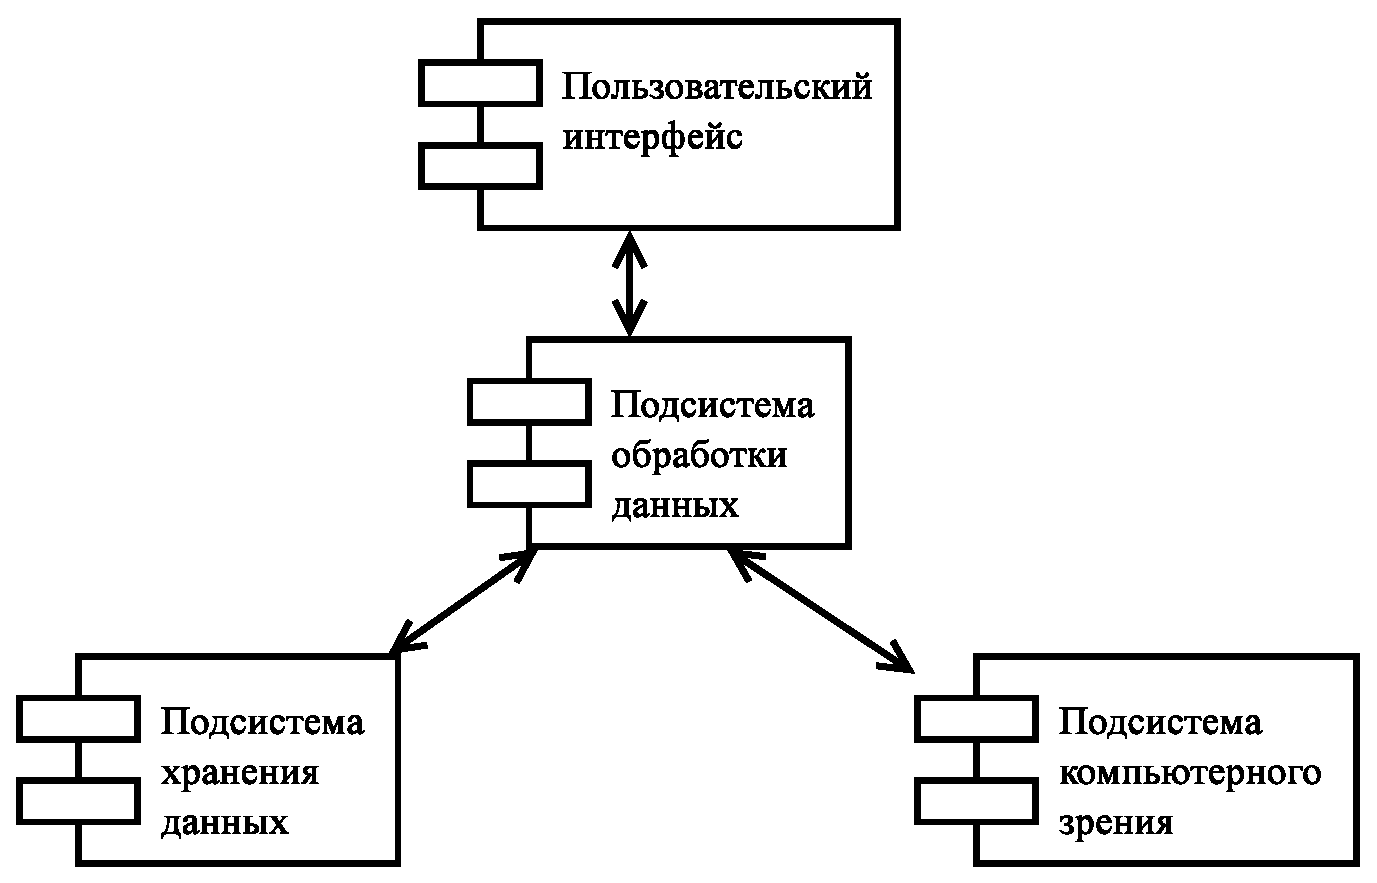
\includegraphics[width=\textwidth]{fig/design_main.eps}
  \end{figure}
\end{frame}

\begin{frame}{Информационное обеспечение}
  Ввод данных:
  \begin{itemize}
    \item ручной;
    \item автоматический.
  \end{itemize}

  \smallskip
  Вывод данных:
  \begin{itemize}
    \item хронологический порядок;
    \item группировка по категориям учета.
  \end{itemize}
\end{frame}

\begin{frame}{Алгоритмическое обеспечение}
  \begin{minipage}{0.6\linewidth}
  Автоматический механизм ввода:
  \begin{itemize}
    \item распознавание числовых данных по изображению с фотокамеры;
    \item метод опорных векторов, гистограммы ориентированных градиентов;
    \item обучение модели классификатора на ПК разработчика.
  \end{itemize}
  \end{minipage}
  \hfill
  \begin{minipage}{0.35\linewidth}
    \begin{figure}[h!]
      \centering
      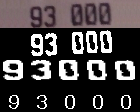
\includegraphics[width=\textwidth]{fig/implementation_cv_recognition.png}
    \end{figure}
  \end{minipage}
\end{frame}

\begin{frame}{Пользовательский интерфейс}
  \begin{minipage}{0.55\linewidth}
    Основные цели:
    \begin{itemize}
    \item удобство использования;
    \item минимум действий при вводе;
    \item соответствие Material Design.
    \end{itemize}

    Результат:
    \begin{itemize}
    \item макеты экранов;
    \item схема переходов.
    \end{itemize}
  \end{minipage}
  \hfill
  \begin{minipage}{0.35\linewidth}
    \begin{figure}[h!]
      \centering
      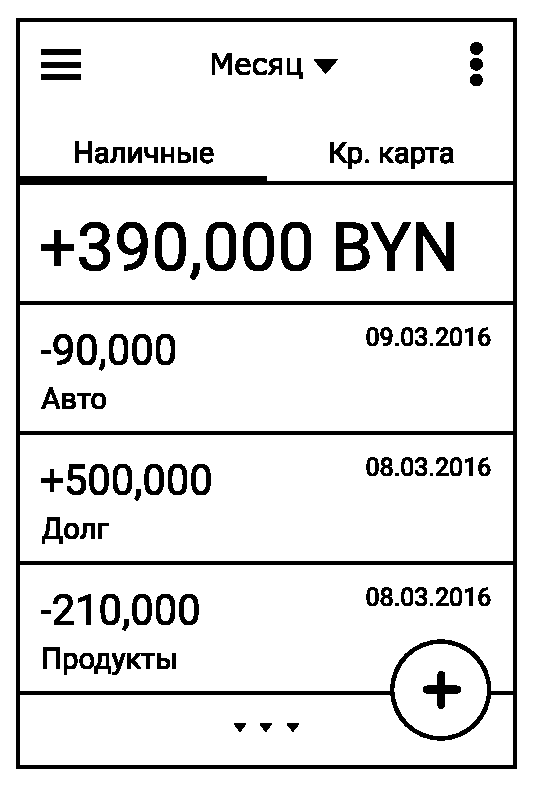
\includegraphics[width=\textwidth]{fig/ui_activities_balance_text_chrono.eps}
    \end{figure}
  \end{minipage}
\end{frame}

\begin{frame}{Детали реализации}
  \begin{itemize}
    \item языки программирования: Java, C++;
    \item СУБД Realm;
    \item \texttt{long} для хранения величин транзакций;
    \item распознавание изображений: OpenCV.
  \end{itemize}
\end{frame}

\begin{frame}{Руководство пользователя}
  \centering
  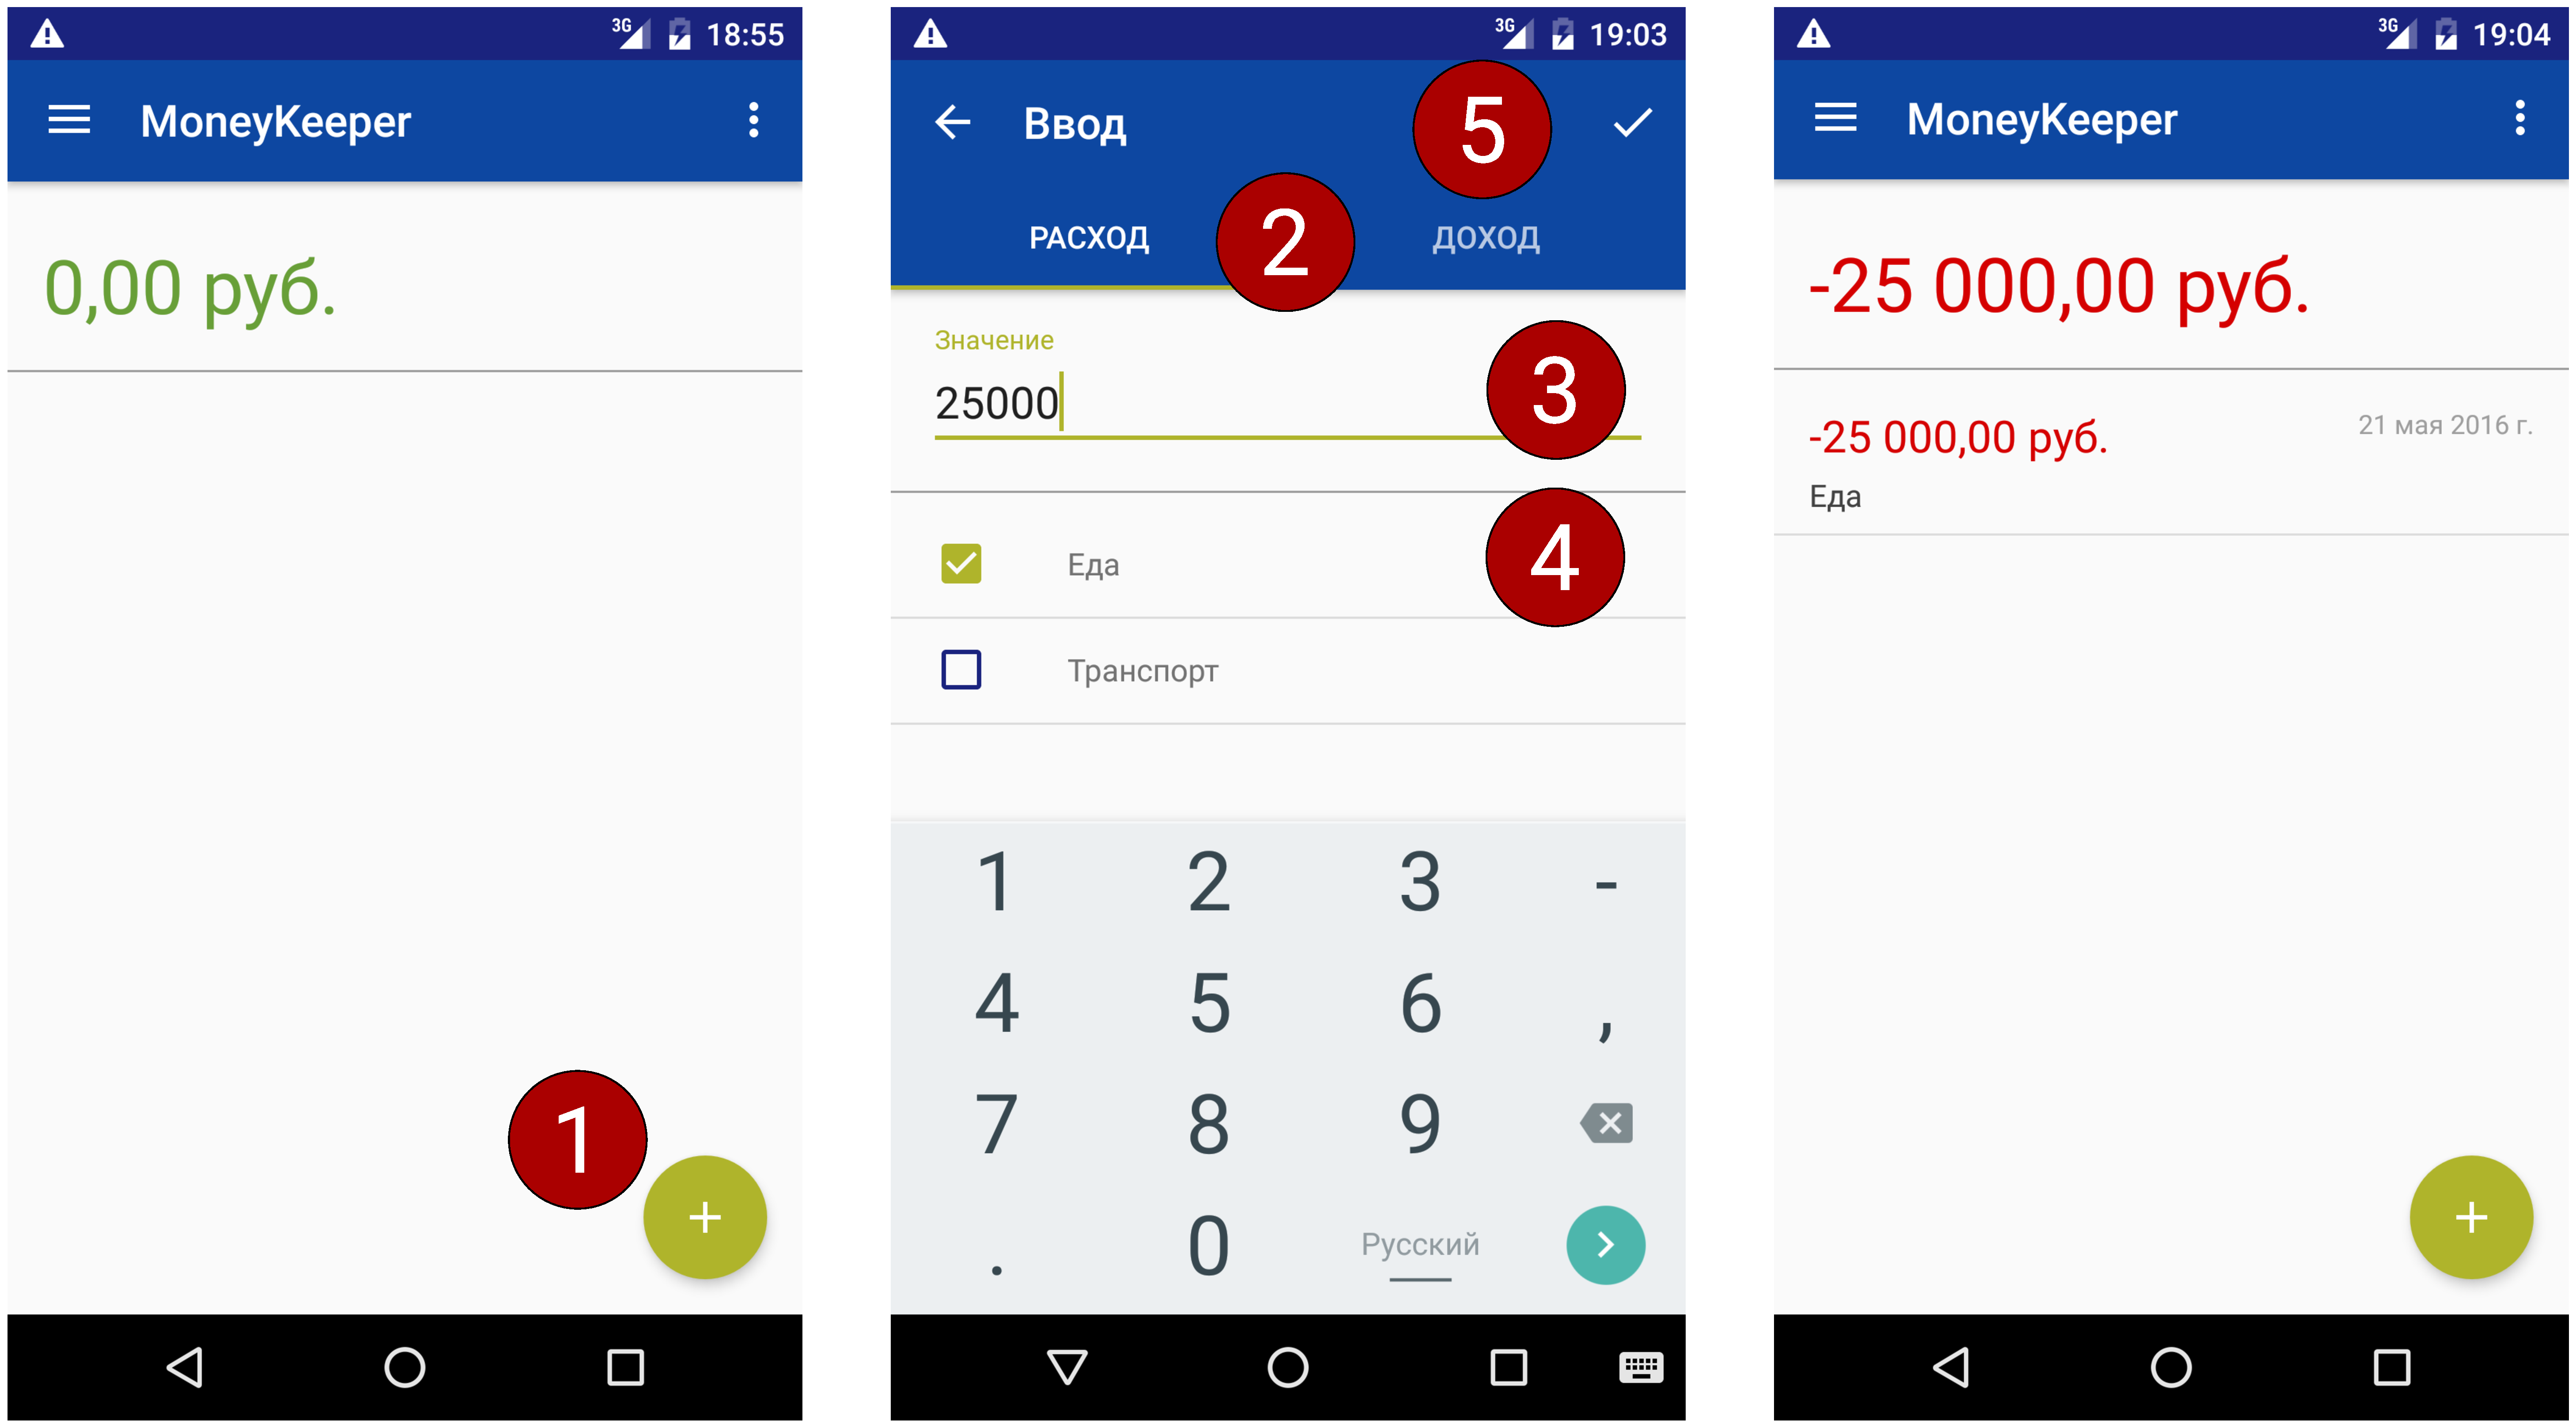
\includegraphics[width=\textwidth]{fig/implementation_manual_balance_change.eps}
\end{frame}

\begin{frame}{Технико-экономическое обоснование}
  Приложение открытое и бесплатное.

  Затраты: \( \approx 184 \) ч., \( \approx 46 \) млн. б. р.

  \smallskip
  Социальный эффект:
  \begin{itemize}
  \item сокращение времени на учет;
  \item анализ затрат \( \Rightarrow \) сокращение затрат.
  \end{itemize}
\end{frame}

\begin{frame}{Перспективы развития}
  \begin{itemize}
  \item повышение точности распознавания числовых данных;
  \item учет переводов денежных средств;
  \item сортировка категорий учета на основании \\
    данных о местоположении.
  \end{itemize}
\end{frame}

\begin{frame}{Выводы}
  \begin{itemize}
  \item ???
  \item исходный код: \url{https://github.com/budnyjj/MoneyKeeper.git}.
  \end{itemize}
\end{frame}

\begin{frame}{Конец}
  \centering
  Спасибо за внимание!
\end{frame}

\end{document}